\chapter{Analysis and solution}
\label{chap:AnalysisAndSolution}
\section{Data analysis}
\label{sec:DataAnalysis}
\subsection{Constructing buildings}
To construct the buildings, we would like to extract data for each building from the BAG data set. However, this data is incomplete. For each building, only a polygon is defined with geographical points. This polygon describes the contour and the exact position of a building. Thus the data contains no information on the height of the building or what kind of roof the building has. In order to determine the height of a building, we can however used the information stored in the residences of a building. For each residence the BAG-dataset contains the total surface area. Combining this with the total area of the surface geometry of a building, we are able to approximate the amount of floors of a building. To approximate the height of a building, we specify that each floor has a height of 2.5 meters. However, for some buildings, only some or no residences are specified, therefore some buildings will get an invalid height. Buildings with no residences will be constructed with an height of 2.5 meters.

Since the bag data set contains no information on the roof, all buildings will get a flat roof. To create the roof for a model cannot be done in a naïve way, since most of the models of the buildings are non-convex polygons. That is, not every point in the polygon is directly visible by all other points, and thus no direct edge can be constructed between two points without the possibility that this edge crosses an edge of the polygon. To produce the roof of a model, an ear slicing algorithm is used. The ear slicing algorithm is a well-known algorithm for triangulating a simple polygon \cite{Kajak11}. The algorithm iteratively locates an ear in the polygon and removes the ear. This process continues till the polygon is a triangle.

A vertex $p_i$ in a polygon is called an ear if the diagonal line between the neighbouring vertexes, $(p_{i-1}, p_{i+1})$, lies entirely within the polygon. That is, this diagonal $(p_{i-1}, p_{i+1}$ does not intersect with any other edge of the polygon. When an ear is found, it is removed from the polygon and the diagonal $(p_{i-1}, p_{i+1})$ will be a new edge within the polygon and the diagonal will be saved in a list. In the end, all the diagonals in the list form the triangulating diagonals for the polygon. An example of a valid ear and the result of the ear-slicing algorithm is shown in figure \ref{fig:ear_slicing}
\begin{figure}[htb!]
    \centering
    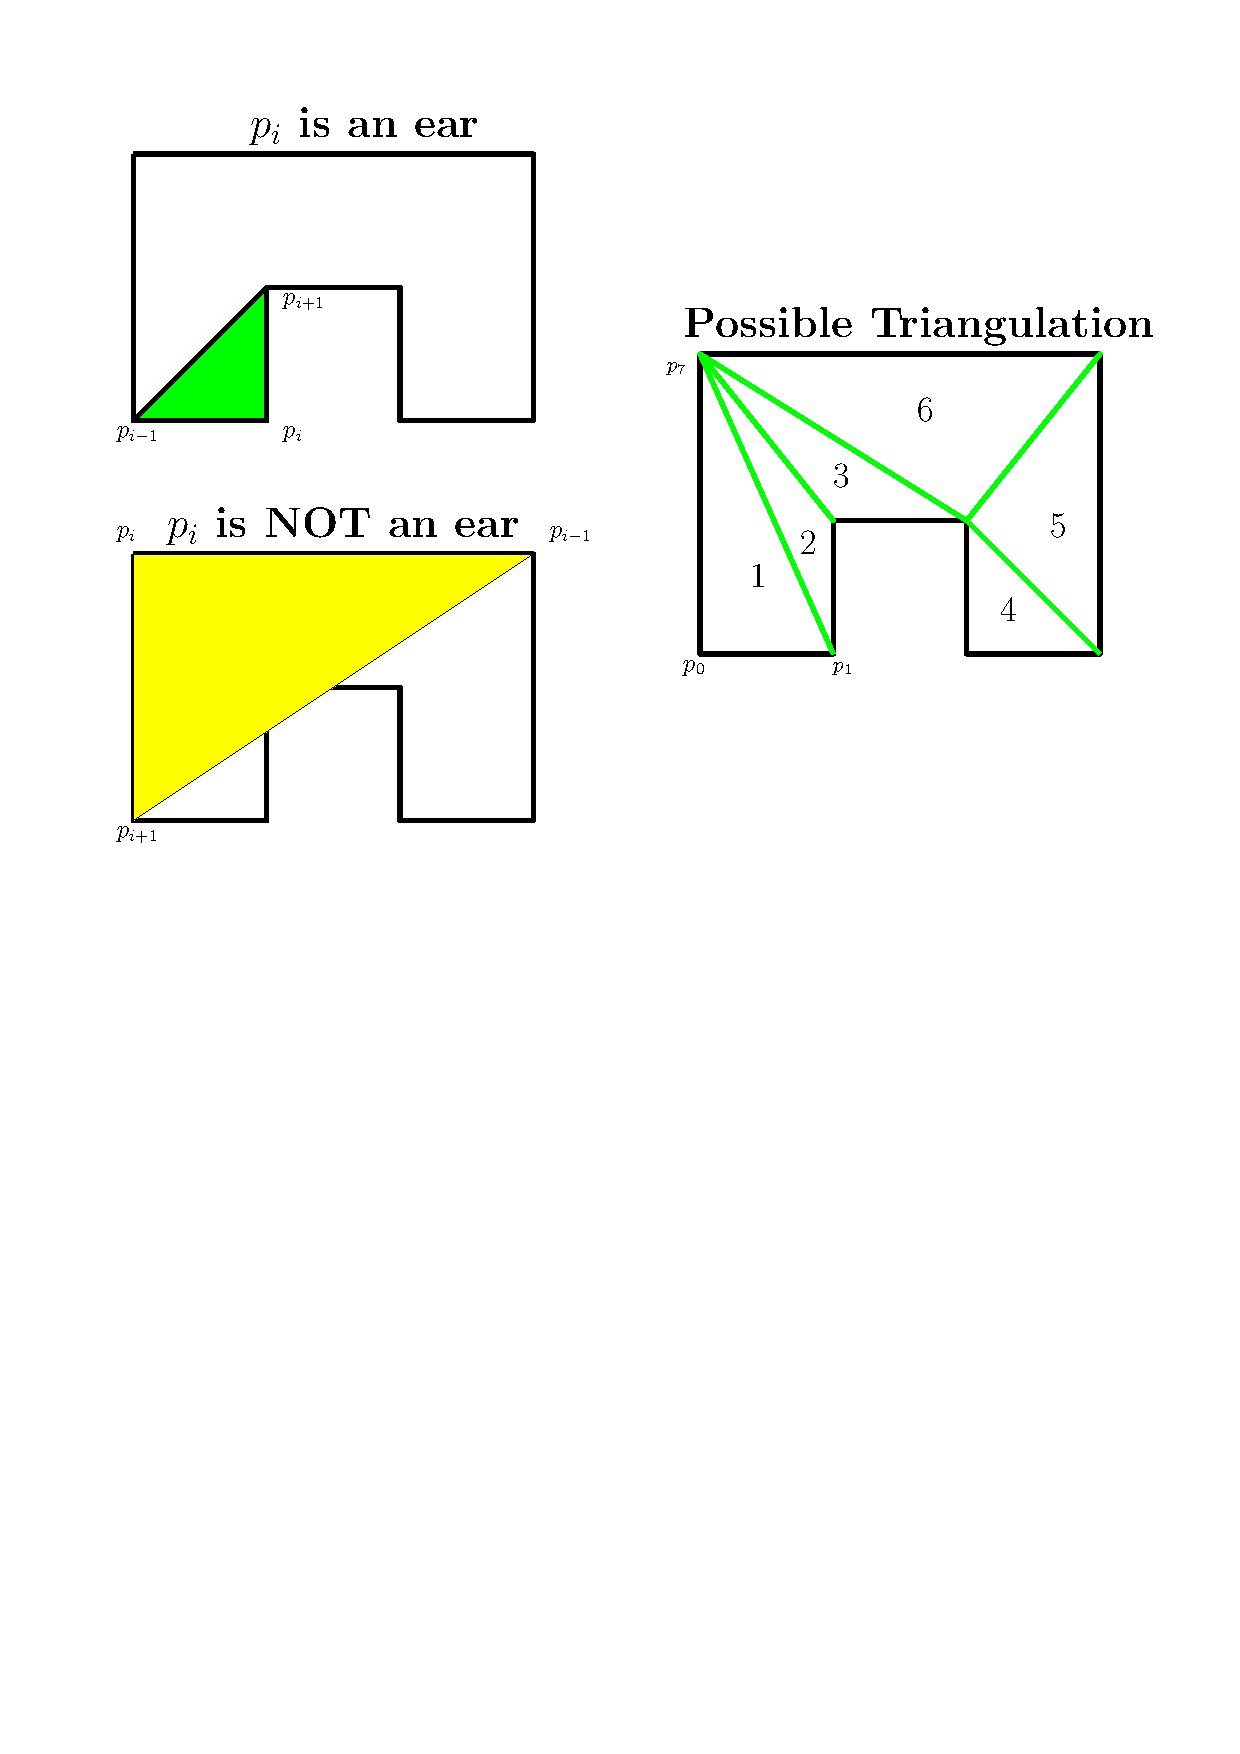
\includegraphics[width=.7\textwidth]{ear_slicing}
    \caption{Example of an ear and ear slicing result}
    \label{fig:ear_slicing}
\end{figure}

\subsection{Constructing roads and surface areas}
We like to use data from OpenStreetMap to construct models of roads, rivers, lakes and other types of surface area. Like described in chapter \ref{chap:OpenDataSets}, a Way in OpenStreetMap describes the position and area of a specific element. Most of Ways also contains a tag. We can use this tag to determine what kind of area the way describes, for example the type of land, water, type of road. If the type is defined in our system, then the system can take the appropriate measures to convert the way into the correct element and apply the corresponding texture. Furthermore, ways can contain meta-information. For example, roads may contain information about the number of lanes. We can use this to approximate the width of a road. For every lane 2.5 meter is used.

\section{System Design}
\label{sec:SystemDesign}
The system is divided in three parts. A global overview of the total system is given in figure \ref{fig:sys_overview}. The first part pre-processes all the data, such that the required data from the BAG and OSM data set is processed to application specific objects, which then are collected in a single data set. For example, the system can process only the data from Eindhoven and remove any unneeded metadata. The second step is the Tree building application. The tree-builder uses the pre-processed data to generate a hierarchy binary tree in which multiple levels of details of all the models is stored. Details of building and using the tree is given in section \ref{subsec:HLOD}. The final part of the application visualises the world. A node manager is used to determine which nodes in the tree needs the loaded into memory and rendered.
\begin{figure}[htb!]
    \centering
    \ifPDFTeX
        \includegraphics[width=.4\textwidth]{SystemDesign.1}
    \fi
    \caption{System overview}
    \label{fig:sys_overview}
\end{figure}

\section{Algorithms}
\label{sec:Algorithms}
\subsection{HLOD}
\label{subsec:HLOD}
Davis \cite{Davis} used a quad tree data structure to check what information has to be rendered on the screen. The leaf nodes contains the most detailed models. The non-leafs contains the combined area of it's childeren, but have a simplified model of the data. With such a data structure it is possible to render further away with less detail.

\subsubsection{Generating HLOD}
Algorithm \ref{alg:CreatingANode} can generate a tree (Where an element is a Building, Road, Grass or Water). In this project we have used this method from Davis, with a single modification that it is possible to use a binary tree. The main advantage over a binary tree is that the split in data can be easily be made data dependent. It is difficult to determine where the split in a quad tree has to be made. In a binary tree it is a trivial choice, to balance the tree the median is used to split the data.

\begin{algorithm}[h]
\caption{Creating a node}\label{alg:CreatingANode}
\begin{algorithmic}[1]
\Procedure{CreateNode}{$E$}\Comment{E = List with elements}
\If{$\Call{TriangleCount}{E} < max_{Triangles}$}
    \State $\Call{CreateModelData}{E}$
    \State \Return $E$
\Else
    \State $E_{splits}\gets \Call{Split}{E}$ \Comment{Split list in 2 or 4 parts}
    \For{$i \gets 1,n_{splits}$}
        \State $E_{splits}[i] \gets \Call{CreateNode}{E_{splits}[i]}$
        \State $E_{compiledList}.\Call{Add}{E_{splits}[i]}$
    \EndFor
    \State $\Call{SimplifyData}{E_{compiledList}}$
    \State $\Call{CreateModelData}{E_{compiledList}}$
    \State $\Return E_{compiledList}$
\EndIf
\EndProcedure
\end{algorithmic}
\end{algorithm}

To simplify data the application merges the 2 elements together to get a more simplified version of the original. This merged version is then again added to the list to merge even further. This algorithm is described in \ref{alg:SimplifyData}. The skiplist used in this algorithm is an custom implementation, where deletes can be done in constant time when holding a reference to the specified item. Earlier version of algorithm \ref{alg:SimplifyData}, it was a simpler algorithm, but for every iteration of the while loop it took $O(n^2)$ time. The update function searched every time for the 2 closest elements. We improved this by keeping for every element the closest element and only searched for a new one if the combination between 2 elements is removed. Also in previous version of the algorithm it used when initializing the skiplist a simple linear search to find the closest element. Which makes the the function $InitilizeSkipList$ an $O(n^2)$ algorithm. Later we found a algorithm that can find the nearest neighbor in $O(\log{n})$ time, with an initialization of $O(n\log{n})$ time. So then the function can run in $O(n\log{n})$ time. The whole algorithm was improved from $O(n^2)$ initial and $O(n^2)$ for every iteration too $O(n\log{n})$ initial and $O(n)$ for every iteration.

Only models of the same type are merged, so for example only buildings are merged with only buildings. The merge is dependent on the type of the element. Buildings are the only type that can be merged at the moment. They are merged with by taking the convex hull of both buildings. Besides the merging of elements, elements are also removed to speed up the process. Small elements like residential roads besides houses are removed low in the tree and large roads like the highways are only removed high up in the tree. This removal is also element dependent. In the current implementation only roads are removed at certain heights of the tree.

\begin{algorithm}[h]
\caption{Simplify data}\label{alg:SimplifyData}
\begin{algorithmic}[1]
\Procedure{SimplifyData}{$E$} \Comment{E = List with elements}
\State \Call{RemoveElements}{E}
\State $n_{triangles} \gets \Call{TriangleCount}{}$
\State $Skiplist \gets \Call{Create}{Skiplist}$ \Comment{Skip list with tuple of elements, sorted on distance}
\State $\Call{InitilizeSkipList}{Skiplist, E}$
\While{$n_{triangles} >= max_{Triangles}$}
    \State $combination \gets Skiplist.\Call{ExtractMin}{}$
    \State $n_{triangles} = n_{triangles} - combination.first.n_{triangles}$
    \State $n_{triangles} = n_{triangles} - combination.second.n_{triangles}$
    \State $E_{newElement} = \Call{Merge}{combination.first, combination.second}$
    \State $n_{triangles} = n_{triangles} + E_{newElement}.n_{triangles}$
    \State $\Call{UpdateLists}{Skiplist, E, combination, E_{newElement}}$
\EndWhile
\EndProcedure
\Function{RemoveElements}{$E$}
\For{$i \gets n,1$}
    \If{$E[i].\Call{NeedsToRemove}{}$}
        \State $E.Remove(i)$
    \EndIf
\EndFor
\EndFunction
\Function{InitilizeSkipList}{$Skiplist, E$}
\State $\Call{BuildKDTree}{E}$
\For{$i \gets 1,n$}
    \State $E_{closest} \gets \Call{KDTreeNN}{E[i]}$ \Comment{Find Nearest Neighbor}
    \State $Skiplist.\Call{Add}{Tuple<E[i], E_{closest}>}$
\EndFor
\EndFunction
\Function{UpdateLists}{$Skiplist, E, combination, E_{newElement}$}
\State For every element $E_{references}$ in $E$ that references 1 of $combination$ call $SkipList.\Call{Remove}{E_{references}}$
\State $E_{closest} \gets \Call{FindNN}{E, E_{newElement}}$ \Comment{Find Nearest Neighbor}
\State $Skiplist.\Call{Add}{Tuple<E_{newElement}, E_{closest}>}$
\State $E.\Call{Add}{E_{newElement}}$
\EndFunction
\end{algorithmic}
\end{algorithm}

\subsubsection{Rendering with HLOD}
We used algorithm \ref{alg:DeterminLoadList} to determine what nodes has to be loaded and unloaded. The decisions are base on a function named CalculateDistanceError. This function is a simple linear function based on the distance to a specified node. The algorithm only returns the differences from the original loaded list and the new loaded list. Most of the time nodes have to be replaced by another single node (when getting farther from the nodes) or a single node needs to be replaced by multiple nodes (when getting closer to the nodes).

\begin{algorithm}[h]
\caption{Determine replace list - Part 1}\label{alg:DeterminLoadList}
\begin{algorithmic}[1]
\Procedure{DetermineReplaceList}{$S, P$}\Comment{$S$ = Current node, $P$ = Position viewer}
    \State $P_{error} \gets \Call{CalculateDistanceError}{S, P}$
    \If{$P_{error} > MaxDistanceError$} \Comment{Too far from the viewer}
        \State $UnloadList \gets newList$
        \State $\Call{DetermineUnloadList}{S, UnloadList}$
        \If{$n_{UnloadList} > 0$}
            \State $ReplaceList.\Call{Add}{EmptyList, UnloadList}$
        \EndIf
    \ElsIf{$P_{error} < S_{error} \And n_{childeren} > 0$} \Comment{$S_{error}$ is too high, descend to childeren}
        \If{$\Call{IsLoaded}{S}$}
            \State $LoadList \gets newList$
            \For{$i \gets 1,n_{children}$}
                \State $\Call{DetermineLoadListForUnloadingParent}{S_{children}[i], UnloadList}$
            \EndFor
            \State $ReplaceList.\Call{Add}{LoadList, S}$
        \Else
            \For{$i \gets 1,n_{children}$}
                \State $\Call{DetermineReplaceList}{S_{children}[i], P}$
            \EndFor
        \EndIf
    \Else \Comment{Load S}
        \If{$\neg \Call{IsLoaded}{S}$}
            \State $UnloadList \gets newList$
            \For{$i \gets 1,n_{children}$}
                \State $\Call{DetermineUnloadList}{S_{children}[i], UnloadList}$
            \EndFor
            \State $ReplaceList.\Call{Add}{S, UnloadList}$
        \EndIf
    \EndIf
\EndProcedure
\algstore{DeterminLoadList}
\end{algorithmic}
\end{algorithm}

\begin{algorithm}[h]
\caption{Determine load list - Part 2}
\begin{algorithmic}[1]
\algrestore{DeterminLoadList}
\Function{DetermineUnloadList}{$S, UnloadList$}
    \If{$\Call{IsLoaded}{S}$}
        \State $UnloadList.\Call{Add}{S}$
    \EndIf
    \For{$i \gets 1,n_{children}$}
        \State $\Call{DetermineUnloadList}{S_{children}[i], UnloadList}$
    \EndFor
\EndFunction
\Function{DetermineLoadListForUnloadingParent}{$S, P, LoadList, UnloadList$}
    \State $P_{error} \gets \Call{CalculateDistanceError}{S, P}$
    \If{$P_{error} > MaxDistanceError$} \Comment{Too far from the viewer}
        \State \Call{DetermineUnloadListForError}{S, UnloadList}
    \ElsIf{$P_{error} < S_{error} \And n_{childeren} > 0$} \Comment{$S_{error}$ is too high, descend to childeren}
        \For{$i \gets 1,n_{children}$}
            \State $\Call{DetermineLoadListForUnloadingParent}{S_{children}[i], P, LoadList, UnloadList}$
        \EndFor
    \Else
        \State $LoadList.\Call{Add}{S}$
    \EndIf
\EndFunction
\end{algorithmic}
\end{algorithm}

Besides the algorithm to determine what has to be loaded, a second algorithm is added that loads the specific nodes. Our fist implementation was a simple version that loads everything in the diff lists, then replaces it with its unloading counterparts, and after that unloads the nodes. This became a problem because, when the list is very long it took a while to load everything. Our second implementation is described in \ref{alg:LoadNode}. This algorithm is run until it doesn't doesn't change the loaded list. In this algorithm we check what has to be loaded and then load only the closest element. This way if loading takes a bit longer than expected, the position is updated while loading the element. For instance if the application is loading Amsterdam, and the user wants to jump to Eindhoven, it isn't still loading Amsterdam, but starts immediately loading Eindhoven. If nodes are only unloaded and not replaced by anything, this can happen if the node is to far from the viewpoint, then it unloads immediately. Unloading can almost be done instantly, so this isn't really a performance issue. We have added that part, berceuse the application has a lower memory footprint.

\begin{algorithm}[h]
\caption{Loading closest node}\label{alg:LoadNode}
\begin{algorithmic}[1]
\Procedure{CreateNode}{$root, P$} \Comment{$root$ = root node, $P$ = Position viewer}
    \State $replaceList \gets DetermineReplaceList(root, P)$
    \If{$n_{replaceList} \> 0$}
        \State $replace \gets \Call{FindClosest}{replaceList, P}$
        \For{$i \gets 1,n_{replace.LoadNodes}$}
            \State $\Call{Load}{replace.LoadNodes[i]}$
        \EndFor
        \For{$i \gets 1,n_{replace.UnloadNodes}$}
            \State $\Call{Unload}{replace.UnloadNodes[i]}$
        \EndFor
        
        \For{$i \gets 1,n_{replaceList}$}
            \If{$n_{replaceList.LoadNodes} = 0 \And \neg (replace = replaceList[i])$}
                \For{$j \gets 1,n_{replaceList[i].UnloadNodes}$}
                    \State $\Call{Unload}{replaceList[i].UnloadNodes[j]}$
                \EndFor
            \EndIf
        \EndFor
    \EndIf
\EndProcedure
\end{algorithmic}
\end{algorithm}


\subsection{Complex polygons}
\label{subsec:ComplexPolygons}
The OSM data is built out of GPS recordings and these recordings have a lot of noise. The noise has the possibility of creating complex polygons in the OSM data. A complex polygon is a self-intersecting polygon. In our OSM data set we have detected multiple complex polygons. This is a problem because the ear-clipping algorithm can only be used for simple polygons. A simple polygon is a polygon that does not contain intersecting edges and does not contain any holes. OSM does not contain any polygons with holes. The detection for a self-intersecting polygons is a naïve algorithm. If two non-consecutive line-segments of a polygon intersect, then the polygon is complex.

To generate a set of simple polygons from a complex polygon, the algorithm has to find two line-segments that intersect. The point at which two edges intersect, two new polygons can be generated. These two new polygons can still be a complex polygon, so the algorithm has to be recursively called on these new polygons. If the input polygon is already simple, then it simply returns the input polygon.

\section{Motivation of choices made}
\label{sec:MotivationOfChoicesMade}
\subsection{Simple polygon test}
\label{subsec:SimplePolygonTest}
Testing if a polygon is simple is done in a naïve way, a faster method is for example the Bentley-Ottmann algorithm \cite{Bentley79}. This algorithm has a running time of $O(\frac{n^2}{\log{n}})$, which is faster that our naïve way with running time $O(n^2)$. We choose the naïve way, since the polygons in the data set are not very large. The largest polygon in the data set containing only Eindhoven had 60 points. Also the time in which we had to develop the application demanded that we used an algorithm that was relative simple to implement.

\subsection{Simple triangulation}
\label{subsec:SimpleTriangulation}
The ear slicing algorithm implemented also has a running time of $O(n^2)$. There also exist algorithms which can triangulate a polygon in $O(n\log(n))$ and $O(n)$ time. These algorithms are however also more complex to implement. And just like for the simple polygon test, our dataset only contains relatively small polygon, therefore longer running times do not form a great constraint.
